\normaltrue \difficilefalse \tdifficilefalse
\correctionfalse
%\UPSTIidClasse{11} % 11 sup, 12 spé
%\newcommand{\UPSTIidClasse}{11}

\exer{Nacelle articule de grande portée $\star\star$ \label{CHS:03:B2:16:84}}
%% 
\setcounter{question}{0}\marginnote{\xpComp{CHS}{03}}%\UPSTIcompetence[2]{B2-16}
\index{Compétence CHS-03}\index{Compétence B2-16}

\index{Nacelle}
\index{Hyperstatisme}

\ifcorrection
\else
\marginnote{\textbf{Pas de corrigé pour cet exercice.}}
\fi


\ifprof
\else
On s'intéresse au châssis d'une nacelle articule de grande portée.

\begin{marginfigure}
\centering
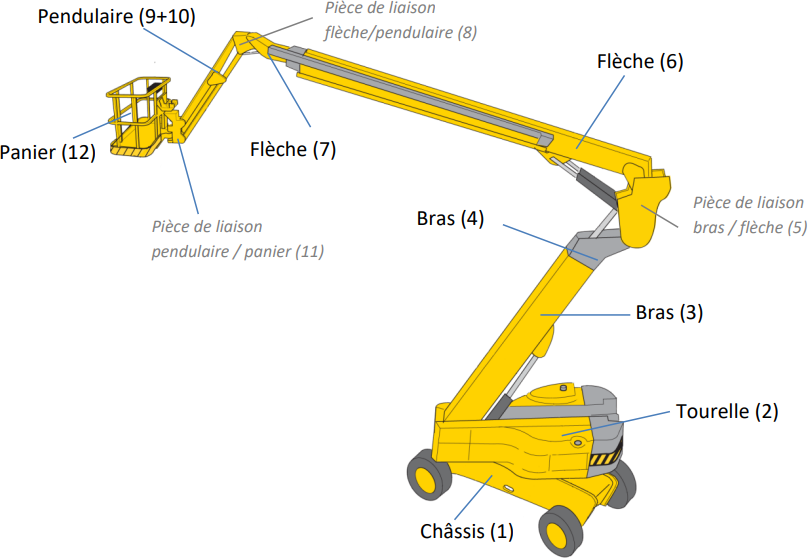
\includegraphics[width=\linewidth]{84_01.png}
%\includegraphics[width=.45\linewidth]{77_02.png}
%\caption{Pince utilisée sur le système ROBOVOLC et schéma cinématique associé \label{fig_23}}
\end{marginfigure} 

La nacelle est amenée à évoluer dans des terrains parfois accidentés (chantier, terrain en friche…).
L’objectif est de valider la motricité du châssis par rapport au sol, même sur un terrain accidenté. 
Le châssis possède un essieu avant monté sur un palonnier pilotable par deux vérins.


\begin{marginfigure}
\centering
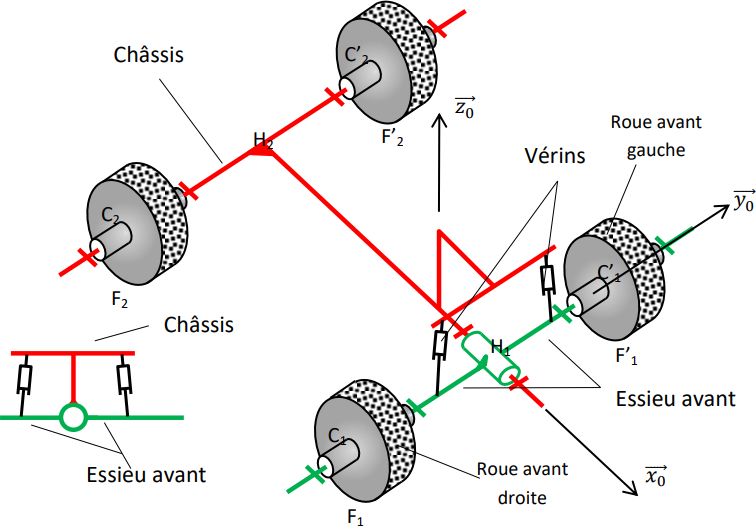
\includegraphics[width=\linewidth]{84_02.png}
%\includegraphics[width=.45\linewidth]{77_02.png}
%\caption{Pince utilisée sur le système ROBOVOLC et schéma cinématique associé \label{fig_23}}
\end{marginfigure} 


$C_1$, $C_1'$, $C_2$, $C_2'$ sont les centres respectivement des roues avant droite, avant gauche, arrière droite 
et arrière gauche. Les quatre roues sont considérées en liaison ponctuelle parfaite avec le sol. Les 
points de contact sont notés respectivement $F_1$, $F_1'$, $F_2$, $F_2'$.

\fi

\question{Déterminer le degré d’hyperstatisme du modèle sans les vérins et 
indiquer si ce modèle permet ou non de conserver le contact avec chacune des roues quelle que 
soit la forme du terrain.}

\question{Déterminer le degré d’hyperstatisme du modèle en faisant l'hypothèse que chacune des extrèmités du vérin est en liaison rotule (avec le châssis et l'essieu).}



Les vérins ne sont toujours pas pris en compte. 

\question{Etablir la liaison équivalente réalisée par le train avant entre le sol et le châssis. 
Donner chaque étape de la démarche.}


\question{ Donner l’avantage de la solution constructeur par rapport à une solution à 4 roues 
directement sur le châssis et par rapport à une solution à 3 roues directement sur le châssis.}


\question{Donner le rôle des vérins et indiquer selon quels critères ils peuvent être pilotés.}


\ifprof
\else

%\noindent\footnotesize
% \fbox{\parbox{.9\linewidth}{
% Éléments de corrigé : 
% \begin{enumerate}
%\item .
%%\item $h=8$.
%\item .
% \end{enumerate}}}
%\normalsize

\marginnote{Corrigé voir \ref{CHS:03:B2:16:84}.}
\fi